\chapter{Résultats et expérimentations}
\label{chapitre.resultats}
	\section{Introduction}
	
	Au cours de ce chapitre, nous pésenterons dans un premier temps le schéma de contrôle en boucle fermé implémenté sur la plate-forme expérimentale.
	Nous présenterons ensuite plusieurs résultats de la loi de commande dévellopée au chapitre \rf{chapitre.commande}.
	Chaque expérience permettra de mettre en évidence un aspect de la loi de commande.
	
	\section{Schéma de contrôle en boucle fermée}
	\label{section.closedloop}
	
	\fig{
		\centering
		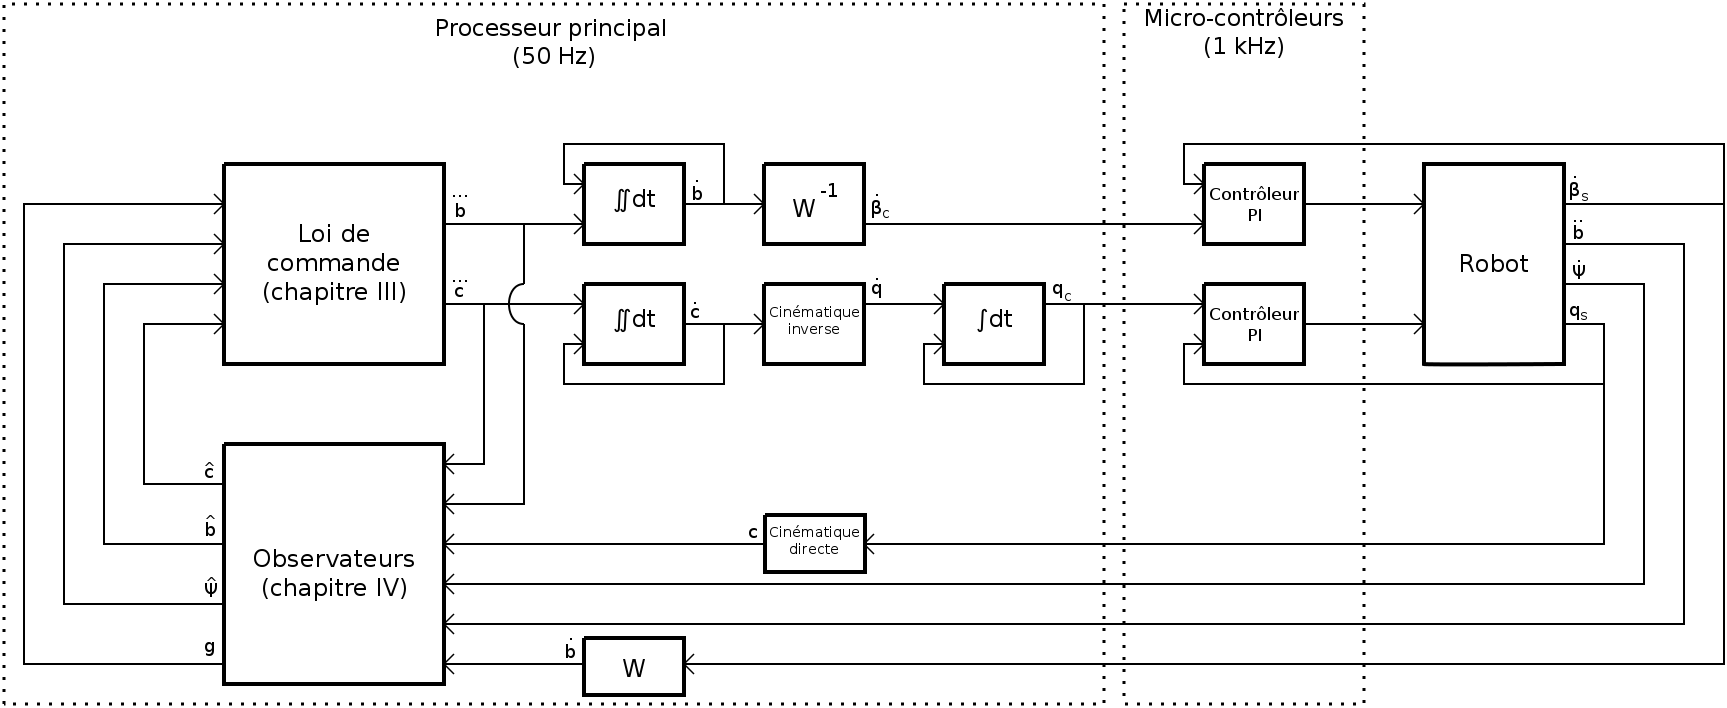
\includegraphics[width=6.5in]{closed_loop.png}
		\caption{Schéma de contrôle en boucle fermée.}
		\label{fig.closed_loop}
	}
	
	L'architecture de commande de la plate-forme expérimentale est séparée sur plusieurs processeurs : 
	Pour chaque moteur, un micro-contrôleur permet de le commander. 
	Un processeur principal permet de réaliser la loi de commande présentée au chapitre \rf{chapitre.commande}.
	
	Dans les sections suivantes, nous détaillerons les différents éléments du schéma de contrôle en boucle fermée \rfi{fig.closed_loop}.
	
	\subsection{Boucle de commande moteur}
	
	  Les micro-contrôleurs commandants chaque moteur sont échantillonés à $1$ kHz.
	  Ils implémentent une boucle de commande de type Proportionnel-Intégral (PI).
	  Ces contrôles sont en position pour les articulations du corps du robot, et en vitesse pour les roues de la base mobile.
	  Les micro-contrôleurs communiquent avec le processeur principal afin de récupérer les réferences en position ou vitesse, puis génèrent une commande envoyée directement aux moteurs.
	  
	  Ces asservissements étant fournis avec la plate-forme expérimentale, il n'a pas été possible de les modifier. 
	  On peut noter que le comportement du robot pourrait être significativement amélioré avec un contrôleur prenant en compte l'accélération et le couple moteur.
	
	\subsection{Boucle de commande principale}
	
	  La boucle de commande principale est échantillonée à $50$ Hz. Elle est séparée en trois éléments :
	  \liste{
	    \item Le premier a pour entrée les données capteurs (vitesses des roues, accélération de la base mobile, angle debasculement et positions articulaires).
		  Les positions articulaires sont converties en position du centre de masse du corps du robot via un calcul standard de cinématique directe, utilisant un modèle du robot.
		  La vitesse de la base mobile est obtenue en multipliant le vecteur des vitesses des roues par la matrice $W$ \rf{eq.obs_beta}.
	    \item Le second élément correspond aux observateurs présentés au chapitre \rf{chapitre.observateur} suivi de la loi de commande du chapitre \rf{chapitre.commande}.
	          Il a pour entrée la sortie du premier élément décrit précédement ainsi que les données de la centrale inertie de la base mobile (accélération de la base et vitesse angulaire).
	          En sortie est obtenu les jerks de commande des CoMs de la base mobile et du corps du robot.
	    \item Le dernier élément permet de convertir les jerks de commande calculés précédements en commandes de position de chaque articulation et de vitesse des roues de la base mobile.
	          Les positions articulaires de commande sont obtenues en intégrant le jerk du CoM du corps du robot puis en résolvant un problème standard de cinématique inverse.
	          Les vitesses des roues sont obtenues en intégrant le jerk du CoM de la base mobile puis en multipliant le résultat par la matrice $\inv{W}$.
	  }
	  
	\subsection{Filtrages capteur}
	
	Quelques filtrages supplémentaires sont nécessaires afin de compenser divers éléments parasites non pris en compte par la loi de commande principale :
	\liste{
	  \item Les mesures des positions articulaire et vitesses capteurs sont quantifiées. 
	        Ainsi, afin de minimiser le bruit de quantification, lorsque la variation entre la mesure actuelle et celle au pas de temps précédent est de l'ordre de grandeur du pas de quantification, alors cette variation est ignorée.
	  \item Le temps de communication entre les capteurs et le processeur principal n'étant pas nul, en ajoutant le retard capteur, les mesures obtenues dans le processeur principal ont un délai conséquent.
	        Afin de le compenser, on extrapole les valeurs capteurs de la façon suivante :
	        \eqa{
		  \tilde{q}_{s_0} &= q_0 + \epsilon_{q_0} \\
		  \epsilon_{q_0} &= q_{s_0} - q_{-\delta}
	        }
	        avec $\tilde{q}_{s_0} $ la mesure extrapolée, $q_{s_0}$ la mesure courante, $q_0$ la commande courante et $q_{-\delta}$ la commande $\delta$ secondes dans le passé, $\delta$ étant le retard de mesure.
	        
	        Ce filtrage suppose que l'erreur entre la commande et la mesure à un moment donné varie peu sur la période $\delta$. 
	        Ainsi, en connaissant cette erreur, on peut estimer la valeur de la mesure courante.
	}
	
	\section{Expériences}
	\subsection{Suivi de trajectoires non réalisables}
	    \subsubsubsection{Protocole expérimental}
	    
	  \fig{
	    \centering
	    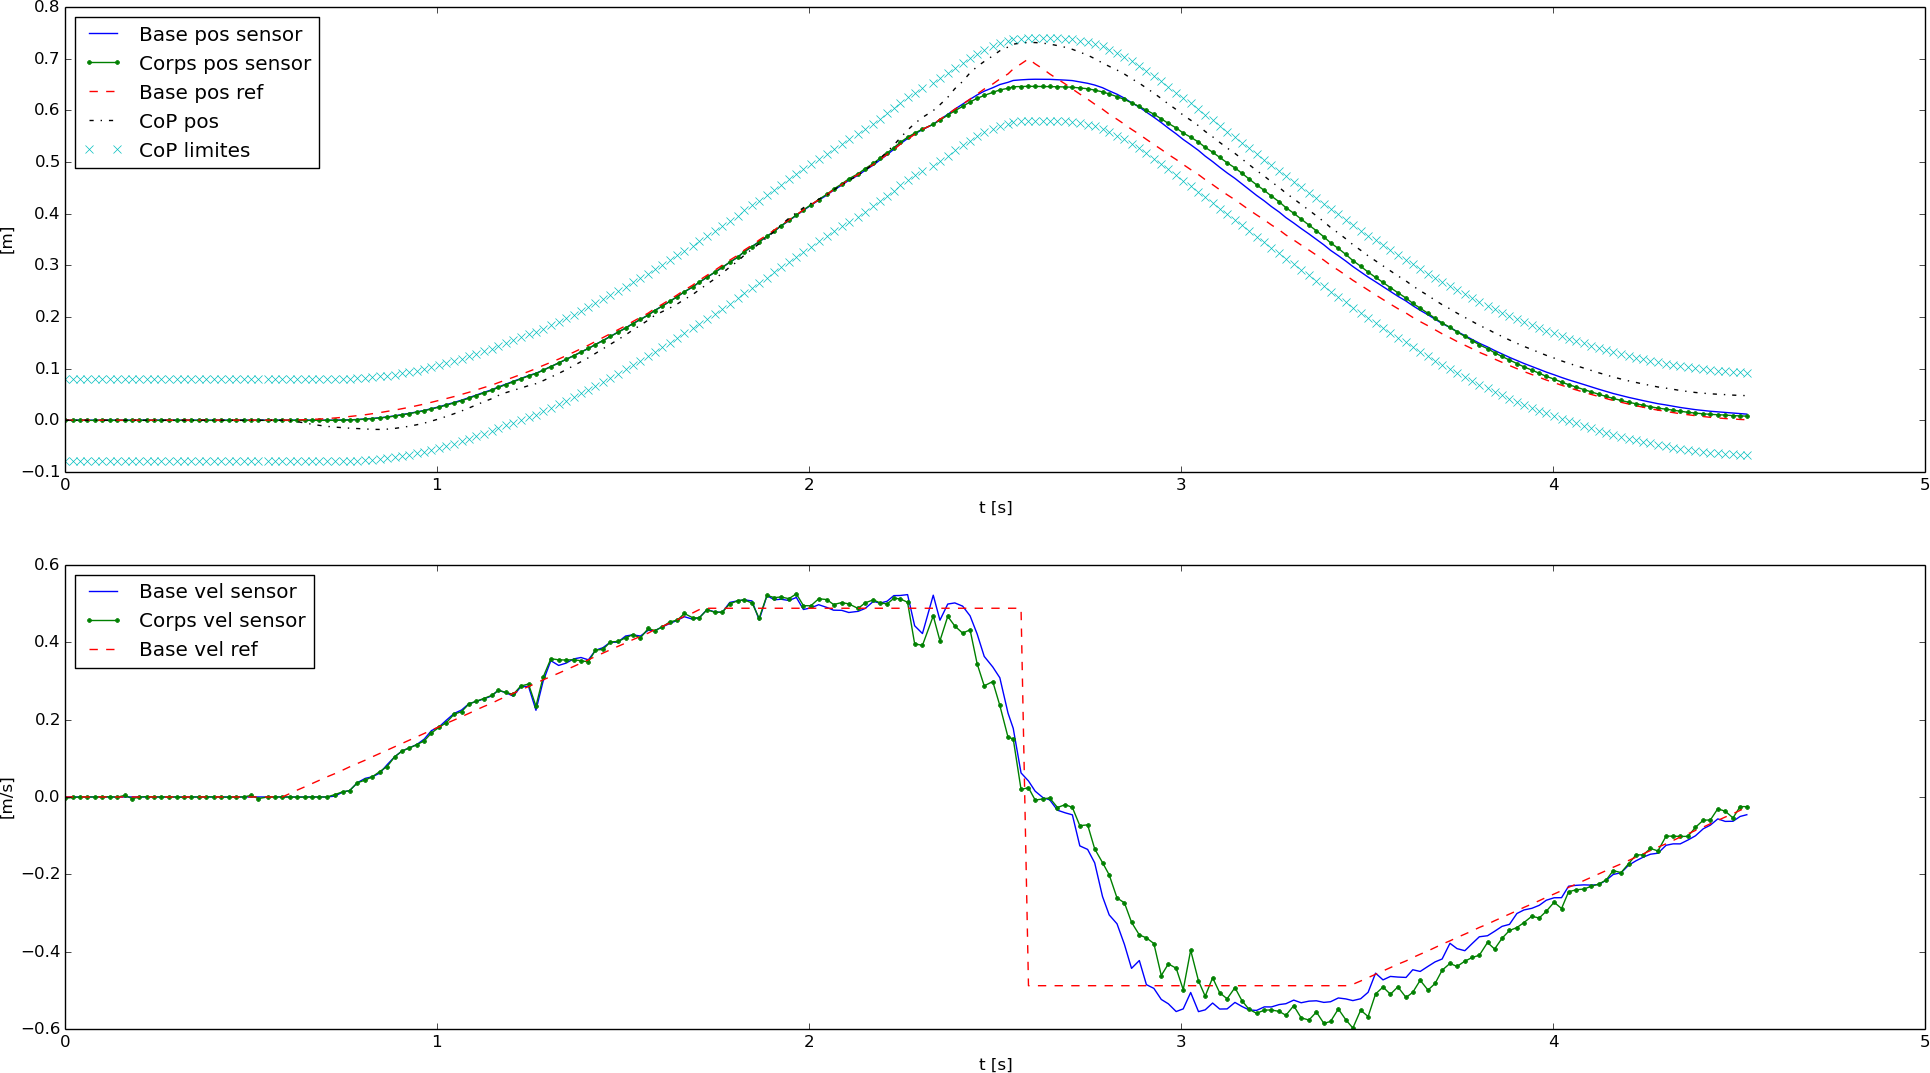
\includegraphics[width=6.4in]{exp1.png}
	    \caption{Suivi d'une trajectoire non-réalisable avec un jeu de pondérations priorisant le suivi de trajectoire par rapport à la robustesse.}
	    \label{fig.exp1}
	  }
	  \fig{
	    \centering
	    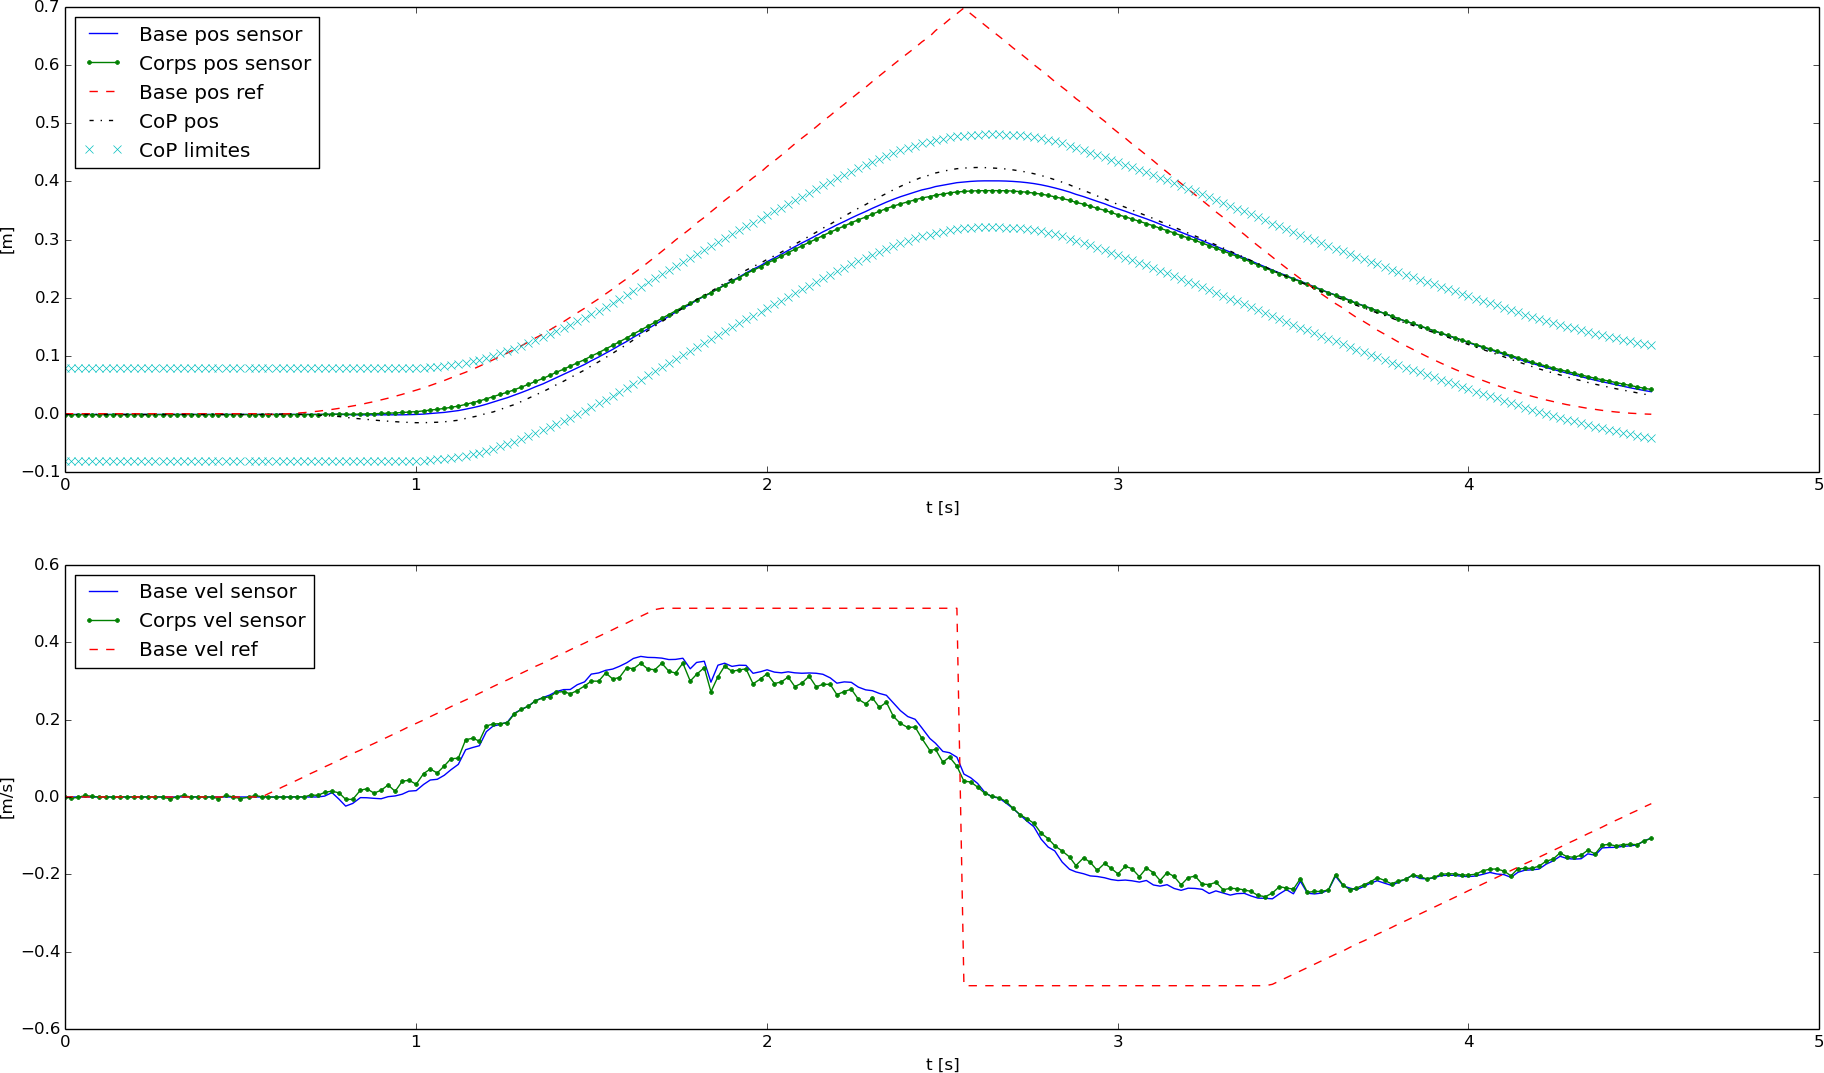
\includegraphics[width=6.4in]{exp2.png}
	    \caption{Suivi d'une trajectoire non-réalisable avec un jeu de pondérations priorisant la robustesse par rapport au suivi de trajectoire.}
	    \label{fig.exp2}
	  }
	  
	  
	      L'objectif de cette première expérience \rfi{fig.exp1}\rfi{fig.exp2} est de montrer l'influence du choix des pondérations dans le comportement de la loi de commande.
	      
	      Le protocole expérimental est le suivant :
	      On dispose le robot les trois roues sur un sol plat et horizontal, en donnant en entrée de la loi de commande une trajectoire de réference non réalisable, avec une discontinuité en vitesse à mi-chemin \rfi{fig.exp1}\rfi{fig.exp2}.
	      La trajectoire consiste en un aller-retour latéral de $70$cm. Celle-ci est dérivable deux fois, exepté à $t=2.6$s où une discontinuité en vitesse à été ajoutée.
	      
	   \subsubsubsection{Analyse}
	    
	    Sur la figure \rfi{fig.exp1}, le jeu de pondérations choisi pour la loi de commande privilégie le suivi de trajectoire vis à vis de la robustesse aux perturbations.
	    Il en resulte une suivi de trajetoire précis.
	    Du fait de l'aspect prédictif de la loi de commande, on peut observer une anticipation de la discontinuité, par une courbure de la trajectoire (et donc une augmentation de l'erreur de suivi instantané) en avance par rapport à la discontinuité.
	    Cette anticipation à pour but de minimiser l'ereur sur l'ensemble de la trajectoire.
	    
	    Le délai de démarrage du mouvement du robot, observé à $t=0.7$s, est dû aux frottements secs situé dans la chaine de transmission entre les moteurs des roues et le sol.
	    
	    On peut noter également que le CoP du robot est proche de ses limites lors de la discontinuité, cela a pour but d'assurer un meilleur suivi de trajectoire, au détriment de la robustesse.
	  
	    Concernant la figure \rfi{fig.exp2}, le jeu de pondérations choisi pour la loi de command privilégie la robustesse aux perturbations vis à vis du suivi de trajectoires.
	    Il en résulte un suivi de trajectoire médiocre, mais une distance entre le centre du robot (position de la base) et le CoP plus faible, ce qui améliore la robustesse.
	    
	\subsection{Suivi de trajectoire en présence de faibles perturbations}
	    \subsubsubsection{Protocole expérimental}
	    
	      \fig{
		\centering
		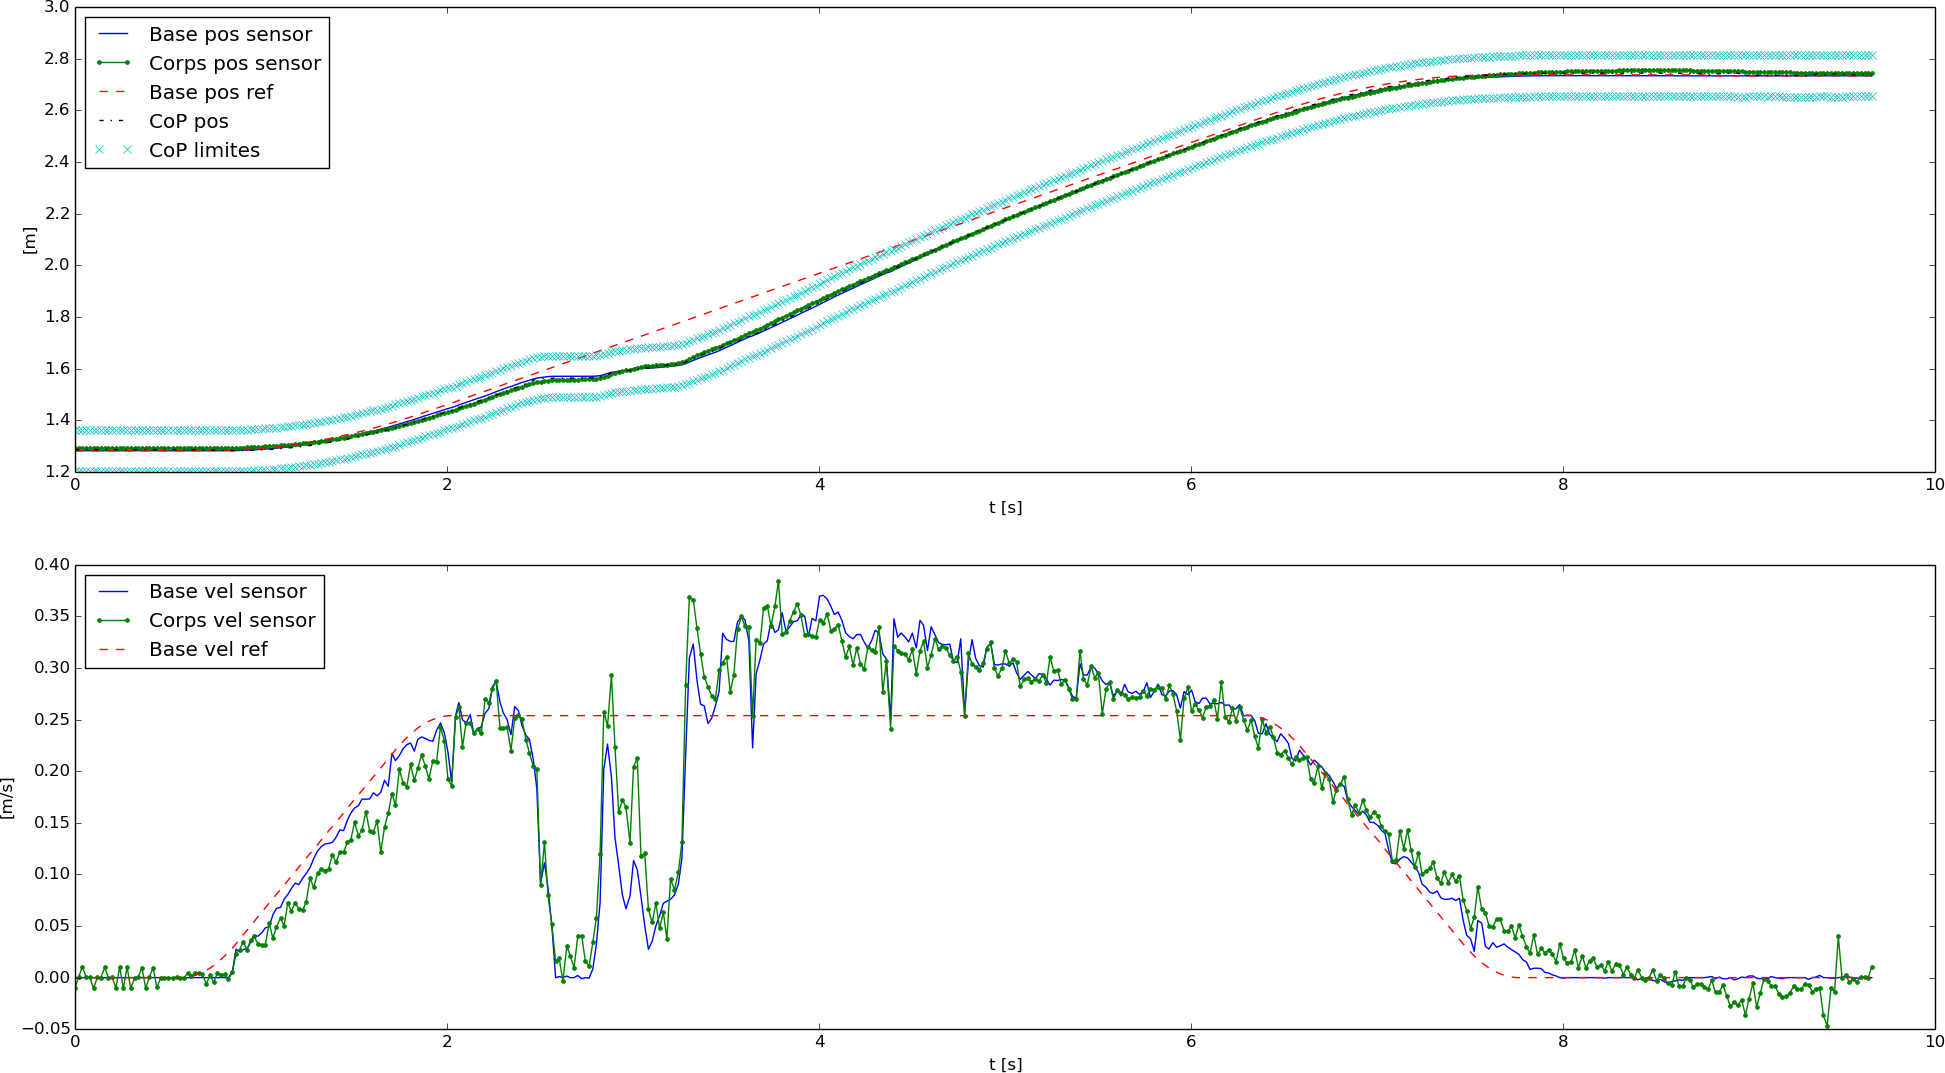
\includegraphics[width=6.4in]{exp6.png}
		\caption{Suivi d'une trajectoire en présence d'une faible perturbation de la base mobile.}
		\label{fig.exp6}
	      }
	      
	      L'objectif de cette seconde expérience \rfi{fig.exp6} est de montrer la capacité de la loi de commande à compenser une faible perturbation de la base mobile.
	     
	      Le protocole expérimental est le suivant :
	      On dispose le robot les trois roues sur un sol plat et horizontal, en donnant en entrée de la loi de commande une trajectoire de réference dérivable deux fois.
	      Celle-ci consiste en un déplacement de $2.8$m vers l'avant.
	      A $t=2.3$s, on perturbe le robot en poussant la base mobile vers l'arrière pendant environs une seconde.
	      
	   \subsubsubsection{Analyse}
	    
	      Sur la figure \rfi{fig.exp6}, on peut dans un premier temps observer la perturbation occasionnée au robot, qui impose une vitesse de déplacement autour de $0$ pendant une seconde environs.
	      Ensuite, afin de rattraper le retard en suivi de position, la loi de commande génère une erreur en suivi de vitesse, en se déplacant plus vite que désiré.
	      La perturbation est compensée à la fois en vitesse et en position en trois secondes environs.
	      
	      L'écart relatif entre les pondérations de suivi en position et en vitesse conditionne le temps de compensation de la perturbation :
	      Si la pondération en suivi de position est très supérieure à celle en vitesse, alors la perturbation sera vite rattrapée. 
	      Si le suivi en vitesse est priorisé par rappport au suivi en position, alors le robot compensera l'erreur en position beaucoup plus lentement.
	      
	    
	\subsection{Compensation du basculement du robot}
	
	  \subsubsection{Lorsque le robot est immobile}
	
	    \subsubsubsection{Protocole expérimental}
	      \fig{
		\centering
		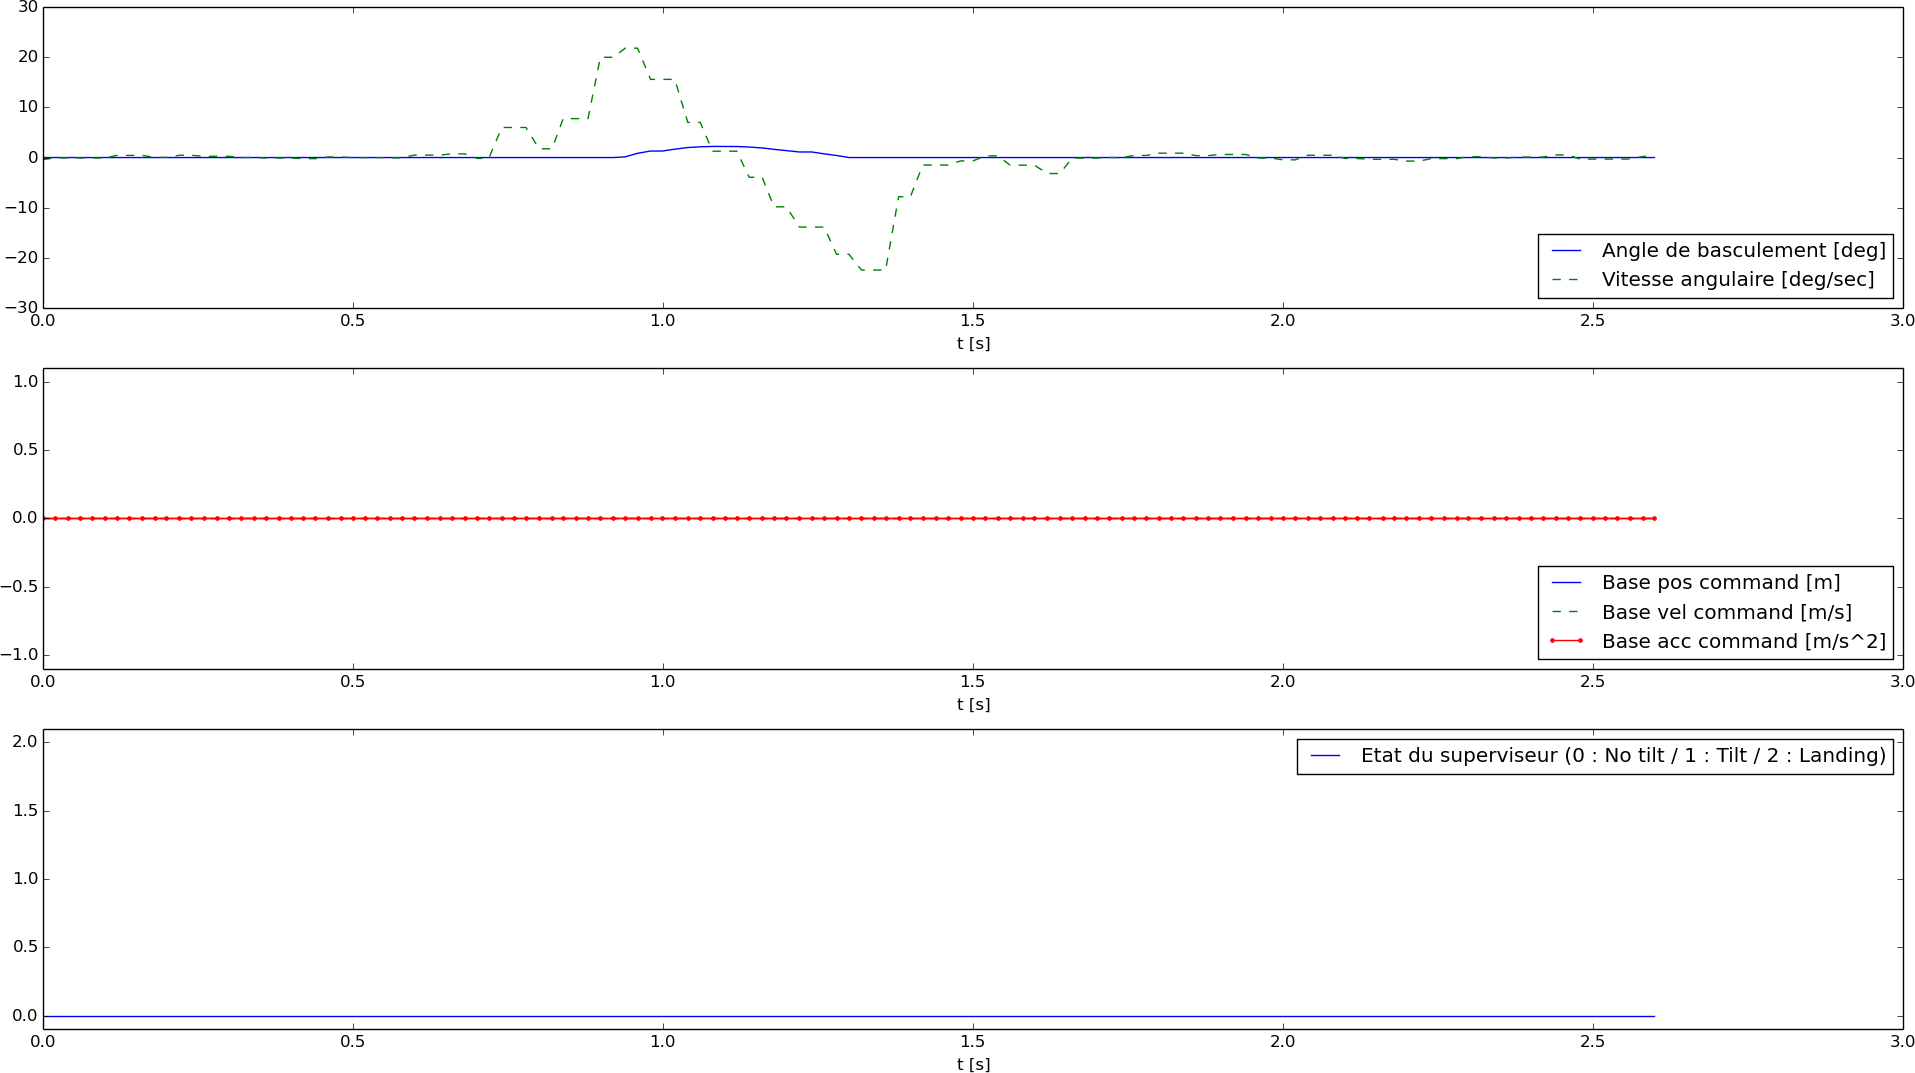
\includegraphics[width=6.4in]{exp3.png}
		\caption{Compensation d'un basculement du robot en présence d'une faible perturbation.}
		\label{fig.exp3}
	      }
	      \fig{
		\centering
		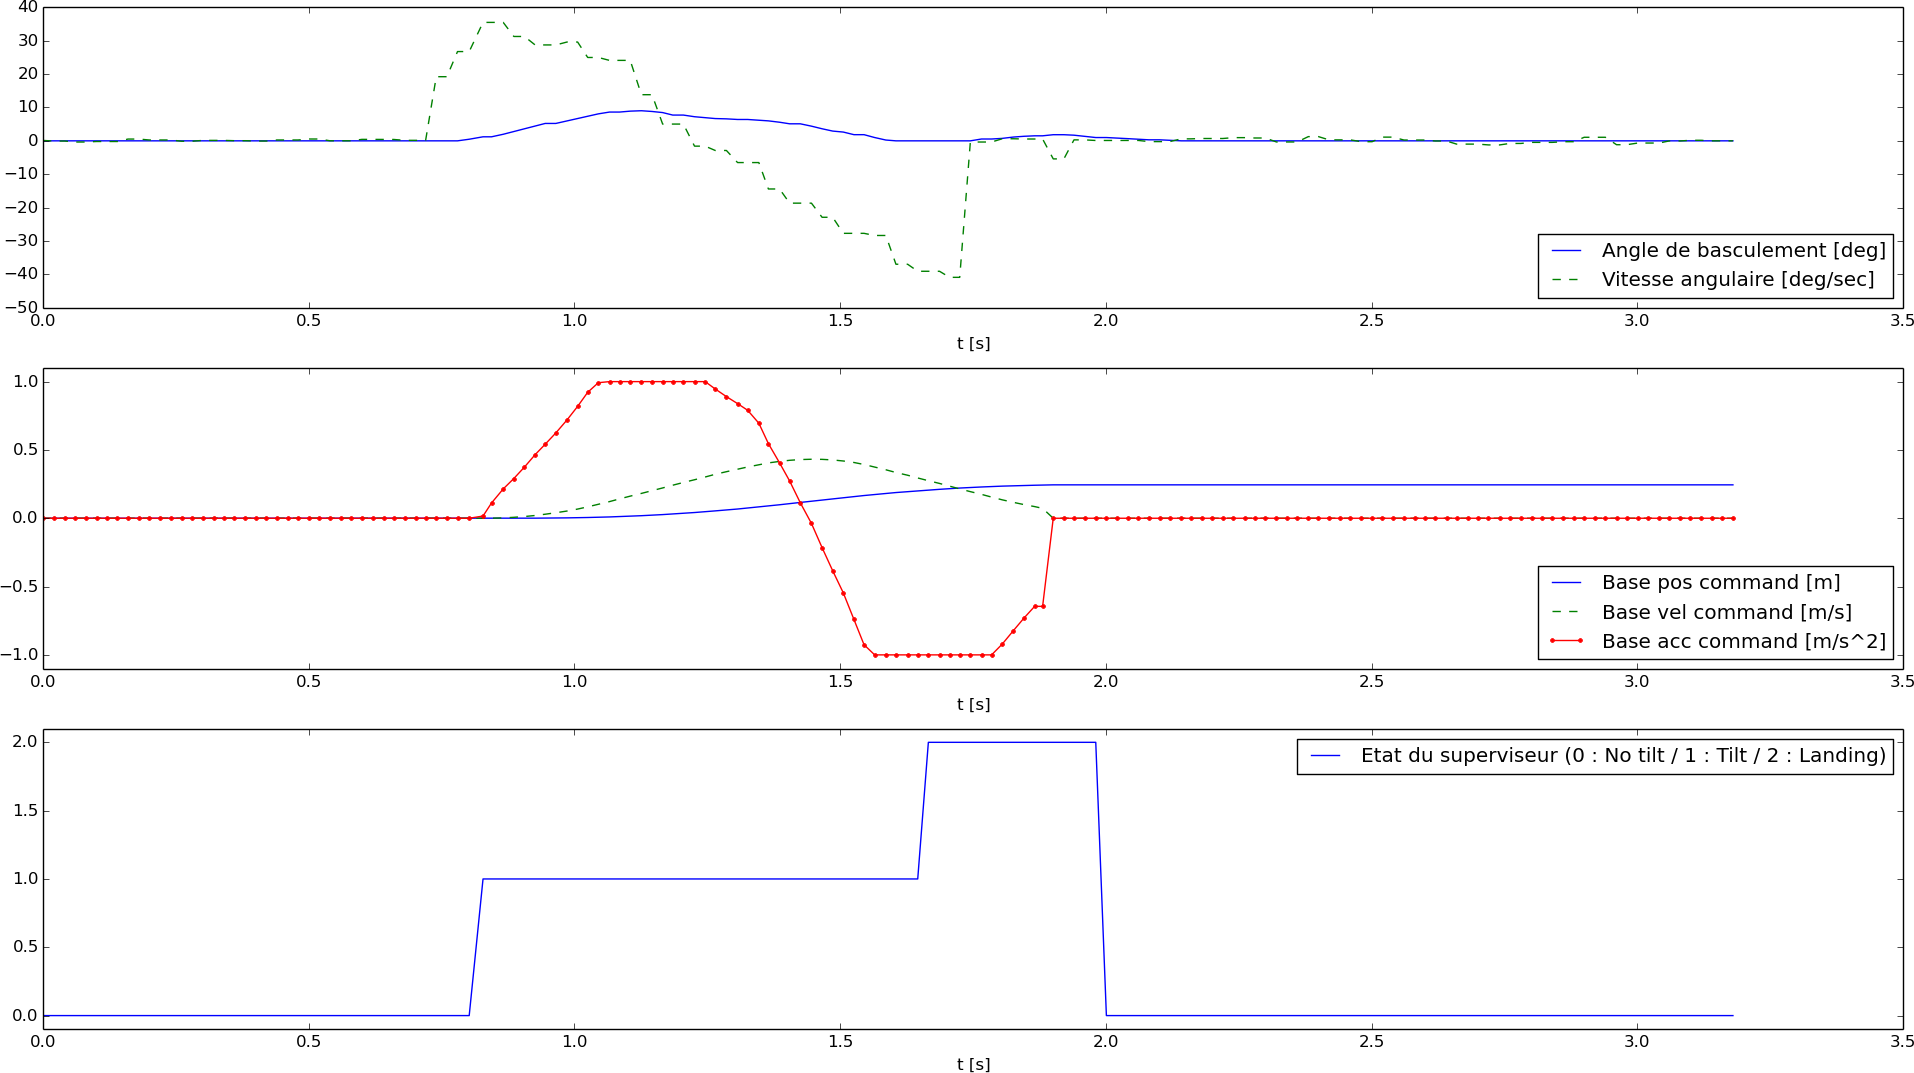
\includegraphics[width=6.4in]{exp4.png}
		\caption{Compensation d'un basculement du robot en présence d'une perturbation moyenne.}
		\label{fig.exp4}
	      }
	      \fig{
		\centering
		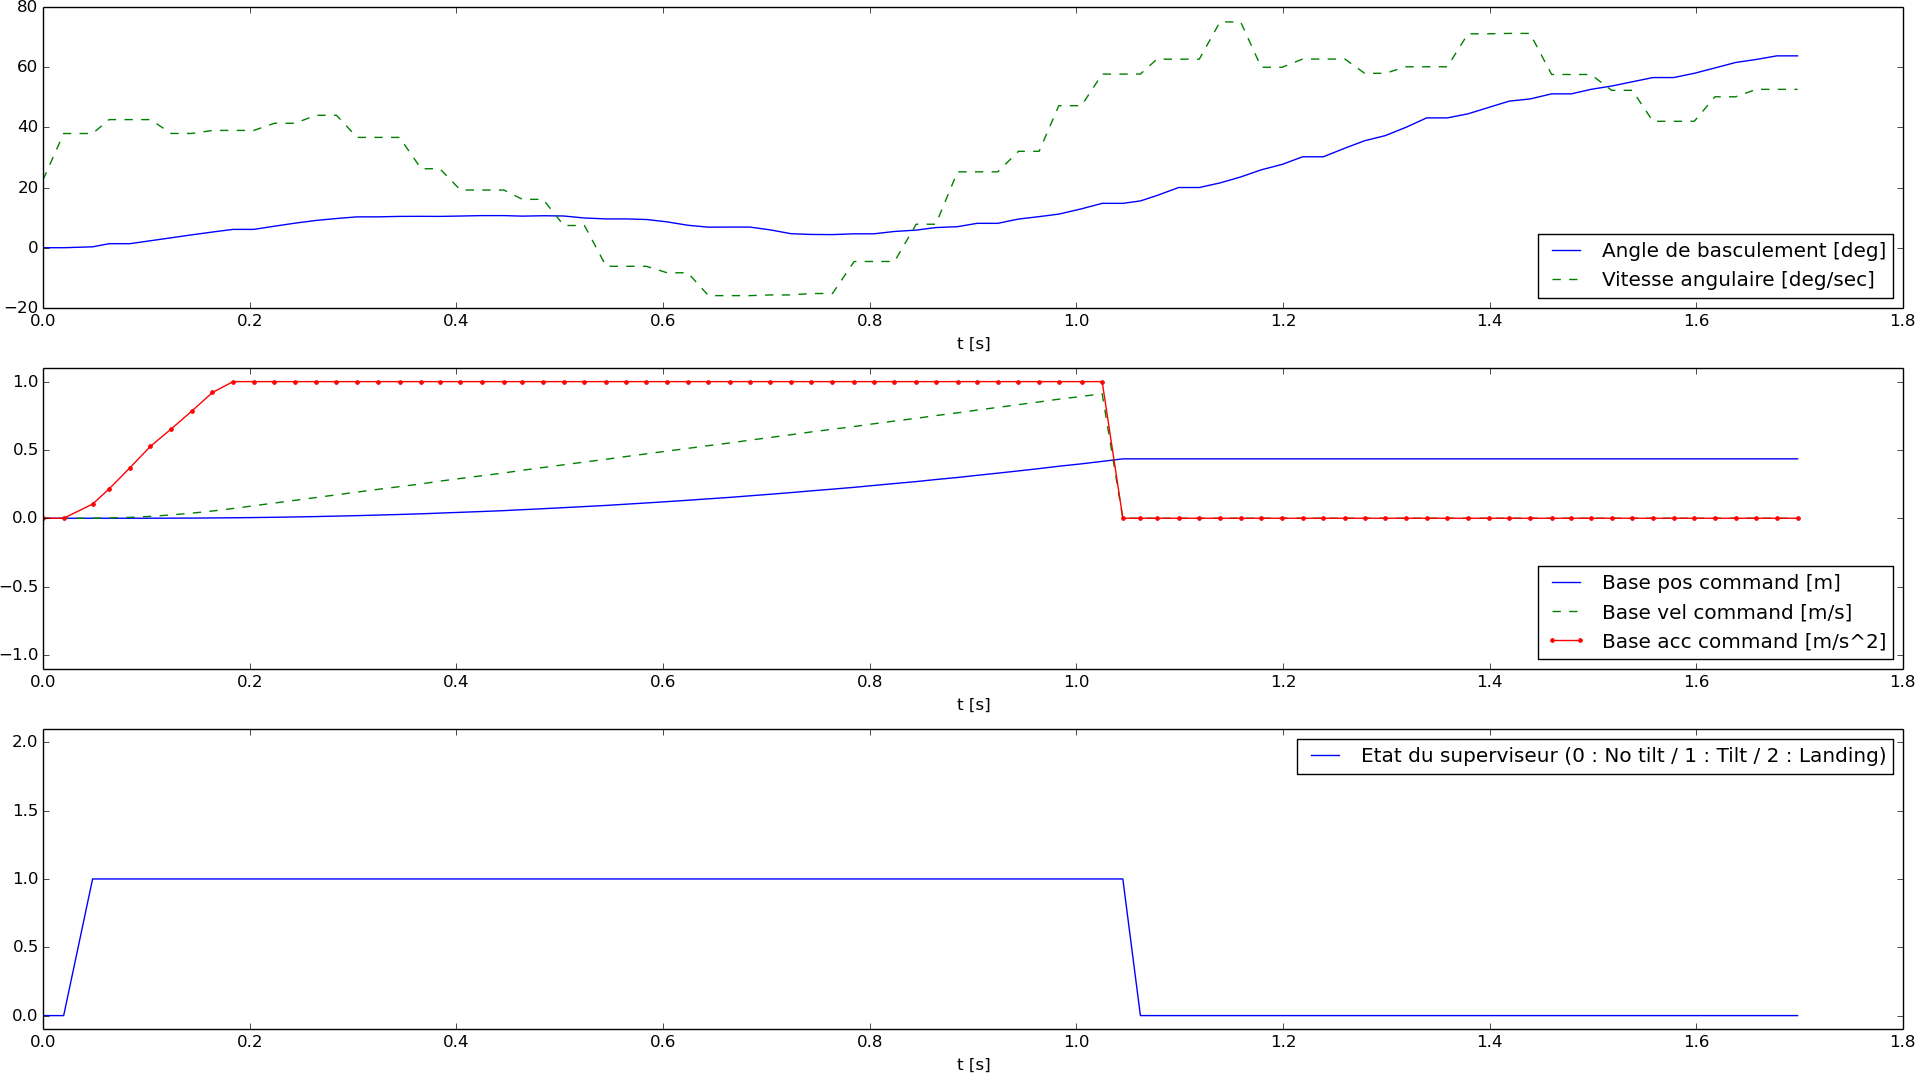
\includegraphics[width=6.4in]{exp5.png}
		\caption{Compensation d'un basculement du robot en présence d'une forte perturbation.}
		\label{fig.exp5}
	      }
	      
	      L'objectif de cette troisième expérience \rfi{fig.exp3}\rfi{fig.exp4}\rfi{fig.exp5} est de présenter le comportement ainsi que les performances de la loi de commande lorsque l'on perturbe le robot de façon à le faire basculer sur deux roues.
	      Dans un premier temps, nous présentons le cas où le robot est initialement immobile.
	      
	      Le protocole expérimental est le suivant :
	      On dispose le robot les trois roues sur un sol plat et horizontal, puis on le pousse par les épaules afin de générer un basculement plus ou moins fort.
	     
	   \subsubsubsection{Analyse}
	     
	     La figure \rfi{fig.exp3} montre l'exemple d'une faible perturbation.
	     Le superviseur possède un seuil limite de vitesse d'impact estimée d'environs $40$deg/s. Celle-ci n'ayant pas été dépassée, la compensation active de basculement n'a pas été déclenchée.
	     La loi de commande a donc laissé la gravité faire atterir le robot à environs $25$deg/s sur le sol.
	     
	     La figure \rfi{fig.exp4} montre l'exemple d'une perturbation moyenne.
	     Dans ce cas, la poussée génère beaucoup de vitesse angulaire, et le superviseur déclenche la compensation active à environs $0.8$s.
	     On observe ensuite des mouvements de la base mobile ayant pour objectif de réduire l'angle de basculement ainsi que la vitesse angulaire au moment de l'impact.
	     
	     La perturbation est compensée en $1$s environs.
	     Il est à noter que la limite en accélération de la base mobile est bornée à $1m$/$s^2$.
	     Si celle-ci était plus grande, les performances seraient meilleures.
	     
	     La figure \rfi{fig.exp5} montre l'exemple d'une perturbation trop forte que la loi de commande est incapable de compenser.
	     Le jerk de commande de la base mobile est saturé dès le début de la compensation (progression linéaire de l'accélération), puis à $0.2$s l'accélération sature à son tour.
	     Avec les limitations actuelles des moteurs de la base mobile, il n'est pas possible de rééquilibrer le robot.
	     Une stratégie de protection contre la chute se déclenche sur le robot à environs $1.05$s, arrêtant toute les commandes envoyées. 
	     
	     
	      
	  \subsubsection{Lorsque le robot est en mouvement}
	
	    \subsubsubsection{Protocole expérimental}
	      \fig{
		\centering
		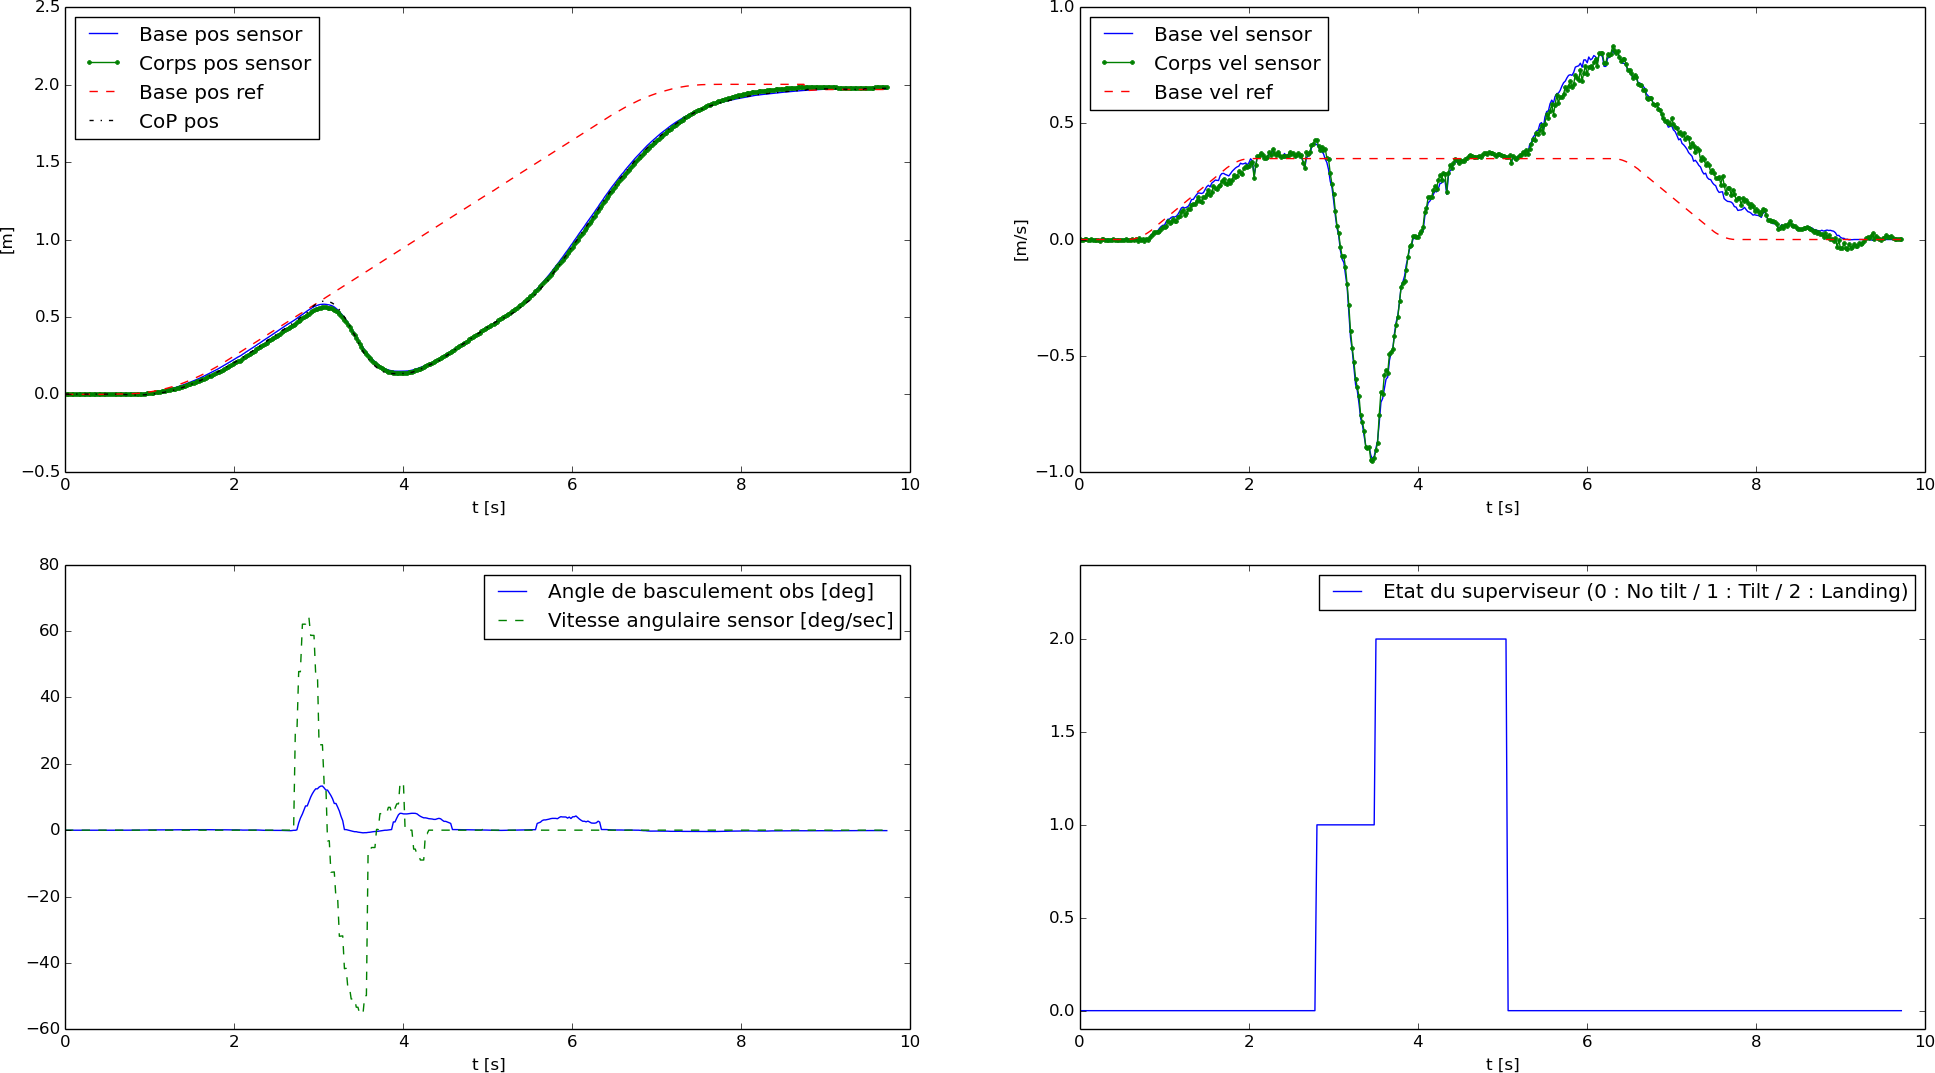
\includegraphics[width=6.4in]{exp7.png}
		\caption{Compensation d'un basculement du robot en présence lorsque celui-ci est en mouvement}
		\label{fig.exp7}
	      }
	      
	      L'objectif de cette quatrième expérience \rfi{fig.exp7} est de présenter le comportement ainsi que les performances de la loi de commande lorsque l'on perturbe le robot de façon à le faire basculer sur deux roues.
	      Nous présentons ici le cas où le robot est initialement en mouvement.
	      
	      Le protocol expérimental est le suivant :
	      On dispose le robot les trois roues sur un sol plat et horizontal, puis on le pousse par les épaules afin de générer un basculement pendant qu'il est en train de se déplacer à vitesse constante.
	     
	      
	   \subsubsubsection{Analyse}
	   
	     Sur la figure \rfi{fig.exp7}, on peut observer que durant la période allant de $2.4$s à $4.5$s, le robot utilise sa base mobile pour compenser le basculement. 
	     Une fois celui-ci rattrapé, on note une forte accélération du robot afin de rattraper son retard en position.
	     
	     Enfin, on peut remarquer deux rebonds après la perturbation initiale (à $4$s et $5.8$s). 
	     Nous avons fait en sorte à ce que la roue en l'air lors de la perturbation ne soit pas motrice (déplacement dans l'axe allant du centre de la roue au centre du robot).
	     Si cela n'avait pas été le cas, les rebonds auraient générés des rotations du robot autour de l'axe $\vec{z}$.
	     Cette situation n'est pas prévue par la loi de commande, et le comportement peut être très instable. 
	     La compensation de basculement dans le cas où le robot bascule est limitée à des perturbations dans la direction du déplacement uniquement.
	      
	\subsection{Compensation de l'inclinsaison du sol}
	
	  
	  \subsubsection{Protocole expérimental}
	    \fig{
	      \centering
	      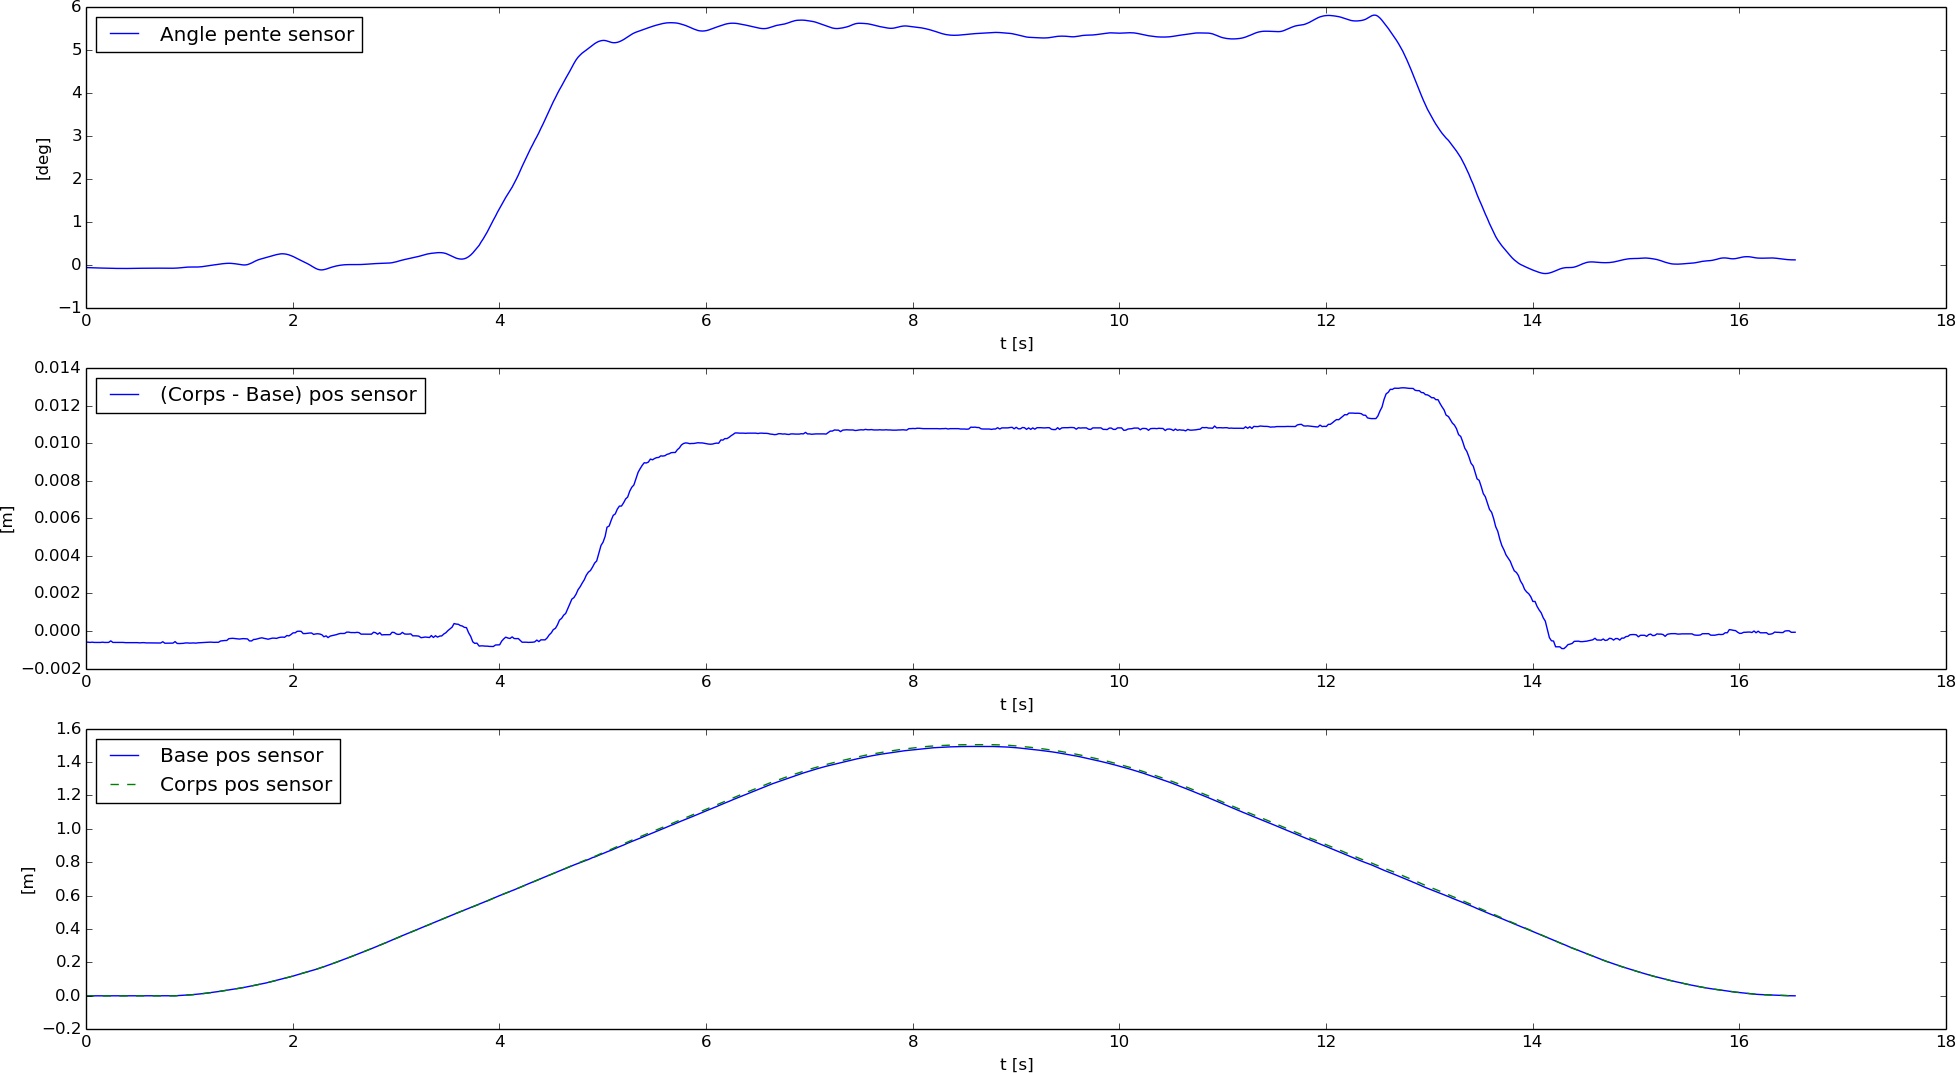
\includegraphics[width=6.4in]{exp8.png}
	      \caption{Compensation de l'inclinaison du sol}
	      \label{fig.exp8}
	    }
	    
	    L'objectif de cette cinquième expérience \rfi{fig.exp8} est de présenter le comportement de la loi de commande lorsque l'inclinaison du sol change.
	    
	      Le protocol expérimental est le suivant :
	      On dispose le robot les troies roues sur un sol plat et horizonal, puis on choisi une trajectoire de référence définie par un aller-retour de $1.5$m en avant.
	      La trajectoire de référence est dérivable deux fois.
	      L'inclinaison du sol change à partir de $0.7$m et devient une pente de $6$ degrés.
	      
	   \subsubsection{Analyse}
	   
	    Sur la figure \rfi{fig.exp8}, on peut observer dans un premier temps que la mesure de l'angle de la pente varie de manière linéaire lors du franchissement de celle-ci. 
	    Cela est dû à la transition au cours de laquelle les roues avant du robot sont sur la pente alors que la roue arrière est sur le sol horizontal.
	    
	    On peut observer également qu'afin de compenser la pente, et de conserver une CoP au centre du robot, la position du CoM du corps du robot se doit d'avancer par rapport à celui de la base mobile.
	    Cette compensation s'opère avec un délai d'environs $0.7$s. Il n'y a pas de compensation en avance de la pente car la valeurs du vecteur gravité n'est pas connue dans le futur.
	    Il y a donc forcément un retard entre la mesure de la pente et la compensation effective de celle-ci par le robot.
	    Cela implique également une limitation de la vitesse du robot lors du franchissement de la pente, afin que le retard généré ne rende pas le robot instable.
	    La vitesse du robot doit également être limités à cause des effets dynamiques dues à la variation de la direction du vecteur gravité, qui n'a pas été pris en compte par la loi de commande.
	    
    \section{Conclusion}  

      Au cours de ce chapitre, nous avons dans un premier temps présenté l'architecture de commande complète du robot. 
      Notament, les effets non pris en compte par la loi de commande ont été filtrés de différentes manières.
     
      Nous avons ensuite présenté diverses expériences, mettant en avant le comportement de la loi de commande dans des situations pertinentes :
      
      La première expérience à consisté à montrer les capacités d'adaptation de la loi de commande à des trajectoires de références non-physiquement réalisables.
      Notament, on a vu que le choix des pondérations est crucial quant-au comportement du robot.
      
      La seconde expérience a permit de montrer les performances de rejet de perturbations de la base mobile.
      
      La troisième expérience a permit de montrer les performances et limitations de la loi de commande à compenser le basculement du robot lorsque celui-ci est initialement à l'arret.
      On peut noter que la dynamique de basculement étant très rapide, il est nécessaire de fournir des accélérations très importantes de la base mobile afin de compenser des perturbations modérées.
      Les performances de compensation du basculement sont principalement limités par les capacités en accélération des moteurs de la base mobile.
      
      La quatrième expérience a permit de montrer les capacités de la loi de commande à compenser le basculement du robot lorsque celui-ci est initialement en mouvement.
      Une forte limitation des performances est la contrainte d'avoir un basculement uniquement dans la direction de déplacement, pour ne pas générer de moment de rotation autour de l'axe $\vec{z}$, qui n'est pas pris en compte par la loi de commande.
      De plus, emmener le robot à basculer dans une direction autre que celle de déplacement conduit à une discontinuité en vitesse de la base mobile.
      
      Enfin, la cinquième expérience a permit de montrer les capacités d'adaptation de la loi de commande à un changement d'inclinaison du sol.
      Ces capacités sont principalement limités par la vitesse de franchissement de la pente, qui ne doit pas être trop grande afin de limiter les effets dynamiques dues au changement de direction du vecteur gravité.
      De plus, l'absence de prédiction de l'inclinaison du sol sur le futur de la trajectoire emmène à compenser le changement de direction du vecteur gravité en retard, ce qui peut conduire à une instabilité de la loi de commande.

